\section{Bug Detector}\label{sec:checker}

\begin{table}
  \centering
  \caption{Type-related specification bugs fixed by pull requests for the recent
  three years from 2018 to 2021.}
  \label{table:pr-bugs}
  \vspace*{-1.5em}
  \[
    \small
    \begin{array}{c|l|r|r}
      \multicolumn{1}{c|}{\textbf{Category}} &
      \multicolumn{1}{c|}{\textbf{Bug Kind}} &
      \multicolumn{1}{c|}{\textbf{\# PR}} &
      \multicolumn{1}{c}{\textbf{\# Bugs}}\\
      \hline

      \multirow{2}{*}{\text{Reference}}
      & \text{Unknown Variables} & \inred{XXX} & \inred{XXX}\\\cline{2-4}
      & \text{Already Defined Variables} & \inred{XXX} & \inred{XXX}\\\hline

      \multirow{1}{*}{\text{Parameter}}
      & \text{Arity Mismatches} & \inred{XXX} & \inred{XXX}\\\hline

      \multirow{1}{*}{\text{Assertion}}
      & \text{Assertion Failures} & \inred{XXX} & \inred{XXX}\\\hline

      \multirow{2}{*}{\text{Type}}
      & \text{Non-Numeric Operands} & \inred{XXX} & \inred{XXX}\\\cline{2-4}
      & \text{Unchecked Abrupt Completions} & \inred{XXX} & \inred{XXX}\\\hline

      \multicolumn{2}{c|}{\textbf{Total}} & \inred{XXX} & \inred{XXX}\\

    \end{array}
  \]
  \vspace*{-1.5em}
\end{table}

% TODO: more detail of investigation

We develop a \textit{bug detector} to statically detect type-related
specification bugs in ECMAScript using an augmented abstract transfer
$\detector$ with additional checkers.  The abstract semantics $\asem{\prog}$ of
a program $\prog = (\getfunc, \getinst, \getnext)$ is the least fixpoint of the
original abstract transfer $\atransfer$.  Thus, $\detector(\asem{\prog})$ also
produces $\asem{\prog}$ and detects type-related specification bugs.  Before
implementing checkers, we manually investigate pull requests for the recent
\inred{three years from 2018 to 2021}.  As described in
Table~\ref{table:pr-bugs}, \inred{XXX} pull requests existed having bugfixes of
\inred{XXX} type-related specification bugs classified in six different kinds
and four categories.  To detect such specification bugs, we implement four
checkers for each category of bugs: \textit{reference checker}, \textit{arity
checker}, \textit{assertion checker}, and \textit{operand type checker}.  Now,
we explain how each checker detects corresponding bugs in the augmented abstract
transfer $\detector$.


\subsection{Reference Checker}

In ECMAScript abstract algorithms, variables are dynamically introduced in any
contexts.  A \textit{reference bug} occurs when trying to access a not yet
defined variable or to redefine an already defined variable.  According to our
manual investigation of pull requests, the reference bug is the most prevalent
type-related specification bugs; \inred{XXX} pull requests fixed \inred{XXX}
unknown variable bugs and \inred{XXX} pull requests fixed \inred{XXX} already
defined variable bugs.  We implement the reference checker by adding additional
checks to abstract semantics of variable lookups $\aseme{\x}$ and variable
declarations $\asemi{\kwlet \; \x = \expr}$ to detect unknown variables and
already defined variables, respectively:
\[
  \small
  \begin{array}{r@{~}c@{~}l}
    \aseme{\x}(\aenv) &=& \left\{
      \begin{array}{ll}
        \text{unknown variable} \; $\x$
        & \text{if} \; \asemr{\x}(\aenv) = \{ \tabsent \}\\
        \cdots
        & \text{otherwise}\\
      \end{array}
    \right.\\

    \asemi{\kwlet \; \x = \expr}(\lab, \tys)(\aelem) &=& \left\{
      \begin{array}{ll}
        \text{already defined variable} \; $\x$
        & \text{if} \; \aty = \{ \true \}\\
        \cdots
        & \text{otherwise}\\
      \end{array}
    \right.\\ &&
    \text{where} \; \aty = \aseme{\x \kwexists}(\aelem(\lab, \tys))\\
  \end{array}
\]
If the abstract semantics of a variable lookup for $\x$ is a singleton $\{
\tabsent \}$, it means the variable $\x$ is always an unknown variable.  In this
case, the reference checker reports an unknown variable bug for $\x$.  For
example, consider the syntax-directed algorithm at the upper-left in
Figure~\ref{fig:example}.  Since the \textbf{GetReferencedName} algorithm is
removed, the variable \code{GetReferencedName} does not exist in abstract
environments and its lookup returns $\{ \tabsent \}$ thus the reference checker
reports the unknown variable bug for \code{GetReferencedName}.  For already
defined variables, the reference checker utilizes the abstract semantics of
existence check $\aseme{\x \kwexists}$ to check whether the variable $\x$ in
each variable declaration is already defined.


\subsection{Arity Checker}

Arity $\size{\func}$ of a function $\func = \kwdef \; \f (\p_1, \cdots, \p_n,
\kwsl \cdots, p_m \kwsr). \; \lab$ is defined as an interval $[n, m]$ where $n$
and $m-n$ denote numbers of normal and optional parameters, respectively.  In
function invocations, an \textit{arity mismatch} occurs when the number of
arguments is not matched with the arity of a function, and \inred{XXX} pull
requests fixed \inred{XXX} arity mismatches.  The arity checker detects such
arity mismatches by using additional checks in the abstract semantics of
function call instructions $\asemi{\x = \kwrl \expr_0 \; \expr_1 \cdots \expr_k
\kwrr}$:
\[
  \small
  \begin{array}{l}
    \asemi{\x = \kwrl \expr_0 \; \expr_1 \cdots \expr_k \kwrr}(\lab,
    \tys)(\aelem) =\\
    \qquad \left\{
      \begin{array}{ll}
        \text{missing parameters} \; \p_{k+1}, \cdots, \p_{n_\func} &
        \text{if} \; \exists \func \in \aty_0. \; \text{s.t.} \; k < n_\func\\

        \text{remaining arguments} \; \expr_{m_\func+1}, \cdots, \expr_k &
        \text{if} \; \exists \func \in \aty_0. \; \text{s.t.} \; k > m_\func\\

        \cdots &
        \text{otherwise}\\
      \end{array}
    \right.\\
  \end{array}
\]
where $\func = \kwdef \; \f (\p_1, \cdots, \p_{n_\func}, \kwsl \cdots,
p_{m_\func} \kwsr). \; \lab \wedge \aty_0 = \aseme{\expr_0}(\aelem(\lab,
\tys))$.  For each function $\func$ in the abstract semantics of the function
expression $\expr_0$, the arity checker compares the number of arguments with
the arity $\size{\func}$ to detect arity mismatches.  For example, consider the
lower-left syntax directed algorithm in Figure~\ref{fig:example}.  The algorithm
invocation in line 2 is compiled to a function call instruction:
\[
  \small
  \x = \kwrl \code{formal}.\code{IteratorBindingInitialization} \; \code{formal}
  \kwrr
\]
with a temporal variable $\x$.  While it passes only a single argument
$\code{formal}$, the arity of the function
$\code{formal}.\code{IteratorBindingInitialization}$ is $[3, 3]$ thus the arity
checker reports missing parameter bugs for two additional parameters
$\code{iteratorRecord}$ and $\code{environment}$.


\subsection{Assertion Checker}
An \textit{assertion failure} is a specification bug that occurs when the
condition of an assertion instruction is not true.  There were \inred{XXX} pull
requests that fixed \inred{XXX} assertion failures.  The assertion checker
detects such bugs using additional checks in the abstract semantics of assertion
instructions $\asemi{\kwassert \; \expr}$:
\[
  \small
  \asemi{\kwassert \; \expr}(\lab, \tys)(\aelem) = \left\{
    \begin{array}{ll}
      \text{assertion failure} \; \expr &
      \text{if} \; \{ \true \} \norder \aty\\

      \cdots &
      \text{otherwise}\\
    \end{array}
  \right.\\
\]
where $\aty = \aseme{\expr}(\aelem(\lab, \tys))$.  It checks whether $\{ \true
\}$ does not have partial order with the abstract semantics of the condition
expression $\expr$.  For example, consider the lower-right syntax directed
algorithm in Figure~\ref{fig:example}.  The parameter $\code{environment}$ of
this algorithm has an environment record or $\undefval$.  Since type sensitivity
divides the abstract types of arguments to upcasted single types, there are two
different abstract environments whose variable $\code{environment}$ points to
$\{ \text{Environment} \}$ or $\{ \undefval \}$.  When $\code{environment}$ is
$\{ \text{Environment} \}$, the abstract semantics of assertion condition
$\code{environment = originalEnv}$ is $\{ \tbool \}$.  Even though we know that
the type of $\code{originalEnv}$ is also $\{ \text{Environment} \}$,
\text{Environment} is not a singleton type thus we cannot convince that they are
the exactly same environment.  Thus, we cannot say that the assertion must be
failed in this case.  However, if $\code{environment}$ is $\{ \undefval \}$, the
abstract semantics of the condition $\code{environment = originalEnv}$ is $\{
\false \}$ because an environment is never equal to $\undefval$.  Thus, the
assertion checker reports an assertion failure for the condition
$\code{environment = originalEnv}$.


\subsection{Operand Type Checker}

\begin{figure*}
  \centering
  \begin{subfigure}[b]{0.24\textwidth}
    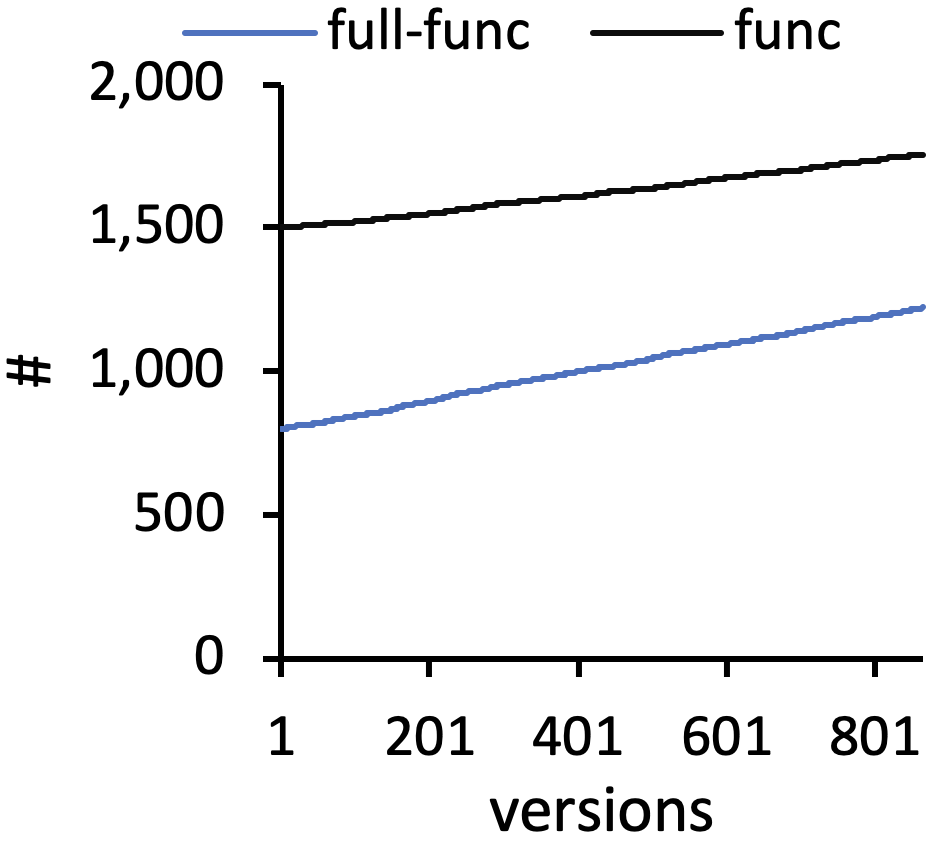
\includegraphics[width=\textwidth]{img/func}
    \caption{The number of functions.}
  \end{subfigure}
  \begin{subfigure}[b]{0.24\textwidth}
    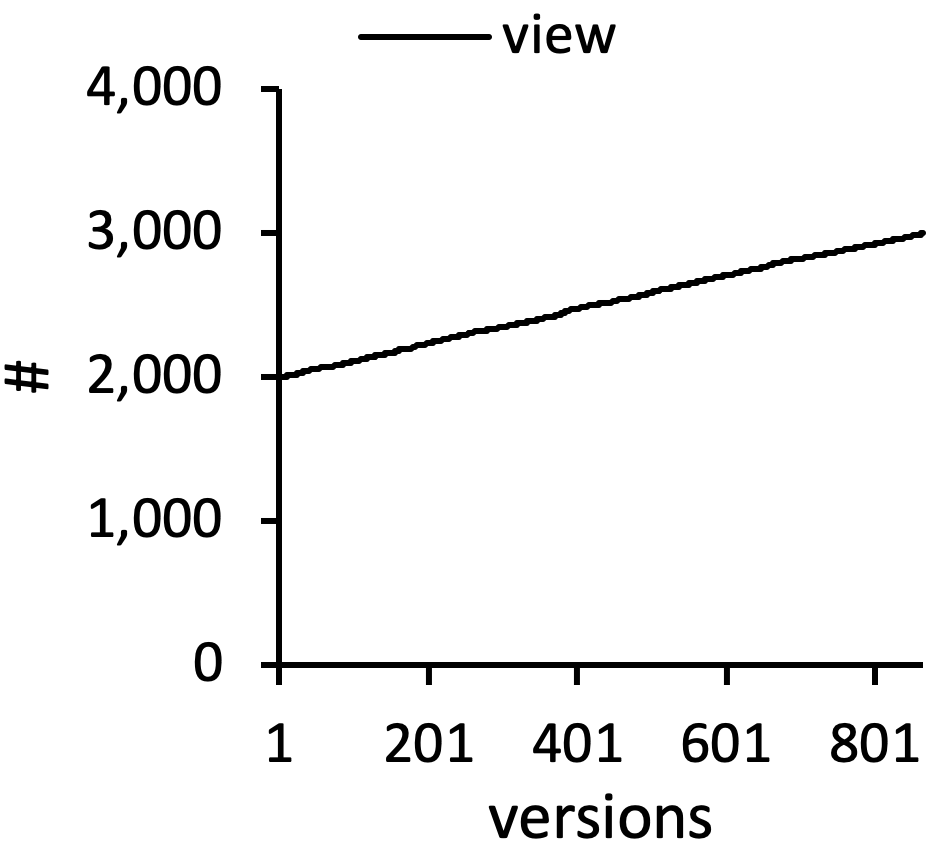
\includegraphics[width=\textwidth]{img/view}
    \caption{The number of views.}
  \end{subfigure}
  \begin{subfigure}[b]{0.24\textwidth}
    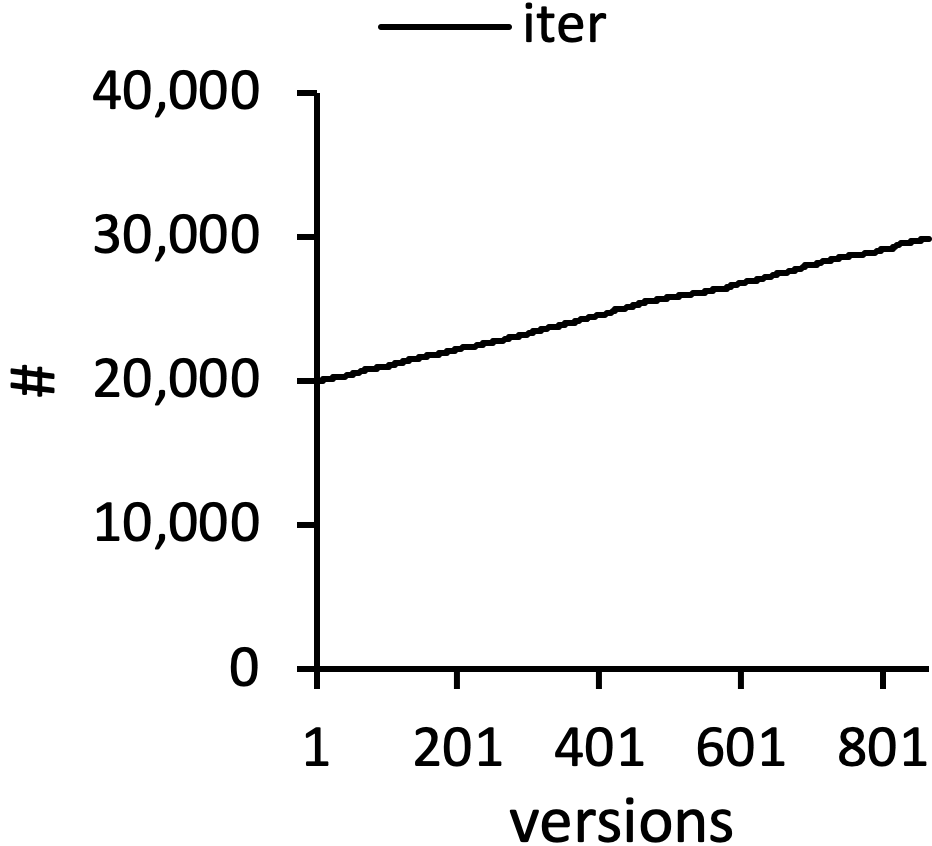
\includegraphics[width=\textwidth]{img/iter}
    \caption{The number of worklist iterations.}
  \end{subfigure}
  \begin{subfigure}[b]{0.24\textwidth}
    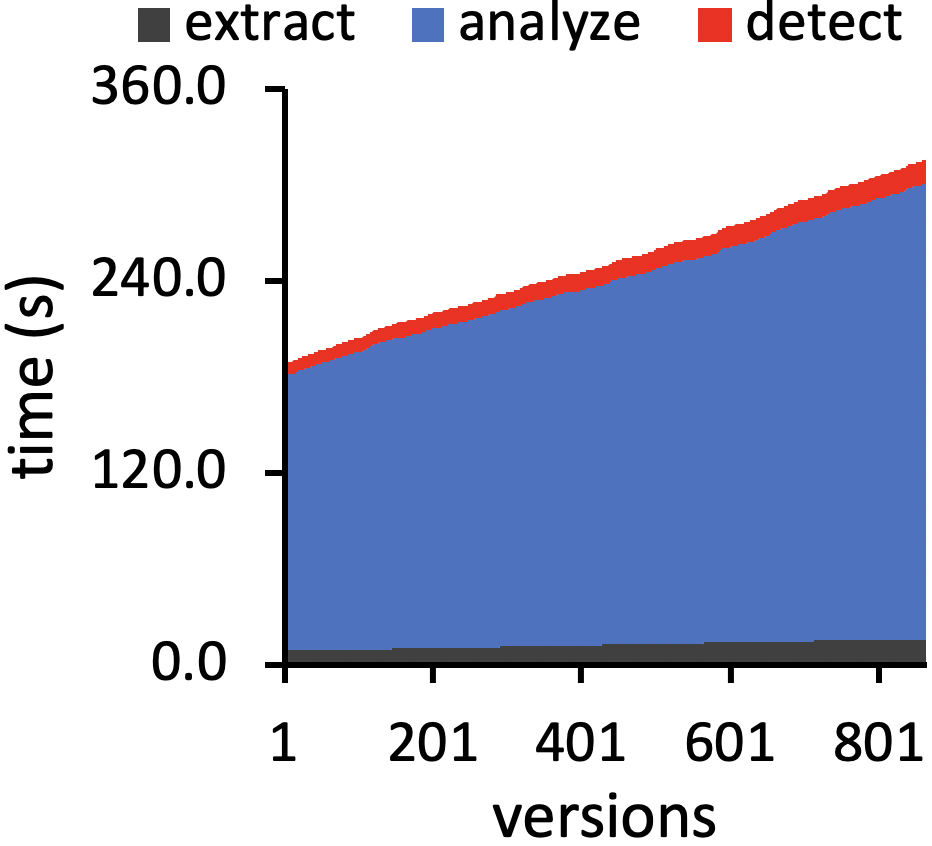
\includegraphics[width=\textwidth]{img/time}
    \caption{The analysis time.}
  \end{subfigure}
  \caption{The statistics of type analysis using $\tool$ for 864 versions of
  ECMAScript.}
  \vspace*{-1.5em}
  \label{fig:stat}
\end{figure*}

Several operators are typed and a \textit{wrong typed operand bug} occurs when
the type of an operand is not conform to the expected type.  For example, the
comparison operator $\code{<}$ is a numeric operator in the modified $\ires$.  If
an expression tries to compare between non-numeric values such as $\true <
\code{"abc"}$, then it is a non-numeric operand bug.  Besides, ECMAScript has a
special implicit conversion for normal completions when their actual values
stored in the $\code{Value}$ field are required including conditions, values of
field updates, operands of operators, etc.  For example, if the variable $\x$
has a normal completion with 42 as its actual value, $\x + 1$ should 43 because
the normal completion implicitly converted into its actual value 42.  To
explicitly represent this conversion, let's define a unary operator $\escaped$:
\[
  \small
  \escaped \val = \left\{
    \begin{array}{ll}
      \val.\code{Value} &
      \text{if} \; \val \; \text{is a normal completion}\\

      \text{unchecked abrupt completion} \; \val &
      \text{if} \; \val \; \text{is an abrupt completion}\\

      \val &
      \text{otherwise}\\
    \end{array}
  \right.
\]
and assume that the operator $\escaped$ is used when the actual value is
required.  Then, an unchecked abrupt completion bug occurs when the actual value
is required but it is an abrupt completion.  According to our manual
investigation, \inred{XXX} pull requests are related to \inred{XXX} non-numeric
operand bugs and \inred{XXX} pull requests are related to \inred{XXX} unchecked
abrupt completion bugs.

The operand checker detects such wrong typed operand bugs by using additional
checks in the abstract semantics of binary operations $\aseme{\expr \bop \expr}$
or unary operations $\aseme{\uop \; \expr}$:
\[
  \small
  \begin{array}{r@{~}c@{~}l}
    \aseme{\expr_0 \bop \expr_1}(\aenv) &=& \left\{
      \begin{array}{ll}
        \text{wrong typed operand} \; \expr_0
        & \text{if} \; \asemr{\expr_0}(\aenv) \norder \aty_0\\
        \text{wrong typed operand} \; \expr_1
        & \text{if} \; \asemr{\expr_1}(\aenv) \norder \aty_1\\
        \cdots
        & \text{otherwise}\\
      \end{array}
    \right.\\

    \aseme{\uop \; \expr}(\aenv) &=& \left\{
      \begin{array}{ll}
        \text{wrong typed operand} \; $\expr$
        & \text{if} \; \asemr{\expr}(\aenv) \norder \aty\\
        \cdots
        & \text{otherwise}\\
      \end{array}
    \right.\\
  \end{array}
\]
where $\aty_0$, $\aty_1$, and $\aty$ are expected abstract types of $\expr_0$,
$\expr_1$, and $\expr$, respectively.  The additional check reports when the
given operand does not conform to the expected types.  For example, consider the
upper-right built-in algorithm $\code{Math.round}$ in Figure~\ref{fig:example}.
The parameter $\x$ has $\{ \tjs \}$ and $\n$ has $\{ \tnum \}$ because the
\textbf{ToNumber} algorithm always return number values or abrupt completions
but later cases are removed by the \textbf{ReturnIfAbrupt} prefix ?.  While the
built-in algorithm correctly uses $\n$ in line 2, it misuses $\x$ in line 3 and
4 and $\{ \tjs \}$ does not have a partial order with the expected abstract type
$\{ \tnum, \tbigint \}$.  Thus, the operand type checker reports non-numeric
operand bugs.
